\documentclass[12pt]{article}

\usepackage[utf8]{inputenc}
\usepackage[T1]{fontenc}  
\usepackage{hyperref}    
\usepackage{url}   
\usepackage{graphicx}
\usepackage{tabularx}
\usepackage{mathptmx}
\usepackage{indentfirst}
\usepackage{subfig}

\graphicspath{ {./graphics/} }

\hypersetup{
	colorlinks=true,
	linkcolor=blue,
	filecolor=magenta,      
	urlcolor=cyan,
}
\urlstyle{same}

\title{\textbf{Rezervări hotele}}

\author{
	Beldiman Vladislav \\ Grupa 1305A
	\\
	Coordonator: Cătălin Mironeanu
}

\renewcommand{\contentsname}{Cuprins}

\begin{document}

\noindent\begin{minipage}{0.1\textwidth}
	
\includegraphics[width=1.1cm]{logo_AC.png}
\end{minipage}
\hfill
\begin{minipage}{1\textwidth}\raggedright
	Universitatea Tehnică "Gheorghe Asachi" din Iași\\
	Facultatea de Automatică și Calculatoare\\
	Baze de Date - Temă
\end{minipage}

\vspace{5cm}
{\let\newpage\relax\maketitle}
\newpage

\tableofcontents
% \newpage

\vspace{4cm}

\section{Descrierea proiectului}

Aplicația dată are scopul de a gestiona baza de date a rezervărilor unui lanț hotelier printr-o interfață grafică ușor de utilizat.

Aceasta asigură o interfață separată pentru clienți și administratorii lanțului.

Cea destinată clienților le oferă posibilitatea de a căuta oferte în perioada dorită, putând fi selectat și orașul, numărul de camere al apartamentului căutat, numărul de adulți și copii, precum și alte opțiuni. Iar, după selectarea unei oferte acesta va introduce datele personale pentru a confirma rezervarea, care implică adăugarea unei rezervări în baza de date, cât și a unui client, dacă nu există.

Cea pentru administrare permite celelalte opțiuni, mai avansate, de actualizare și ștergere în toate entitățile, și adăugarea unui oraș, hotel sau apartament.

În plus, aplicația șterge clientul din baza de date atunci când nu mai are nici o rezervare.

\newpage

\section{Tehnologii folosite}

\begin{itemize}
	\item Front-end
	
	Qt

	\item Back-end

	Python și Oracle Database

\end{itemize}

\section{Structura și inter-relațioarea tabelelor}

\begin{figure}[!htb]
	\centering
	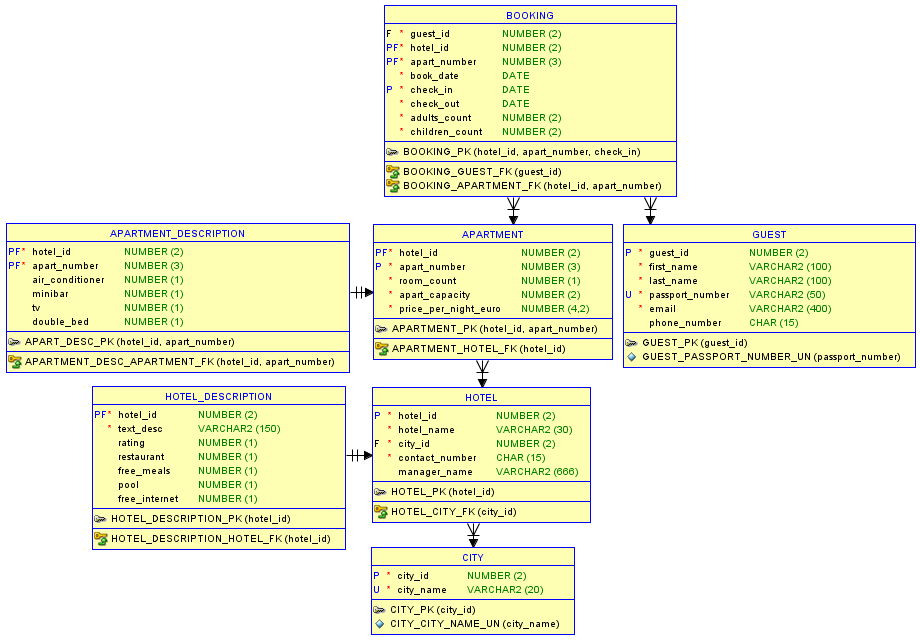
\includegraphics[width=\linewidth]{Relations.PNG}
	\caption{Diagrama ER.}\label{fig:fig1}
\end{figure}

Entitatea BOOKING și relațiile one-to-many afterente ei au fost obținute în urma normalizării relației many-to-many dintre entitățile GUEST și APARTMENT.

\section{Constrângeri}

Am folosit id-uri ca primary key pentru a facilita actualizarea entităților. Entitatea BOOKING nu are un id drept primary key, deoarece nu există foreign key-uri la niciuna din atributele sale.

Constrângerile de tip unique au fost folosite pentru a putea realiza toate operațiile fără a folosi explicit id-urile, care sunt redundante.

Foreign key-urile sunt folosite pentru a lega entitățile între ele.

Atributele air\_conditioner, minibar, tv, double\_bed, restaurant, free\_meals, pool și free\_internet pot avea doar valorile 0 sau 1 prin care e subînțeles False sau, respectiv, True, deoarece sunt folosite doar pentru a confirma existența acestor facilități.

Apart\_capacity și adults\_count pot lua valori în intervalul 1 - 20 inclusiv, iar children\_count: 0 - 19, deoarece copii trebuie însoțiți. De asemenea, există constrângerea children\_count + adults\_count <= apart\_capacity care e singura constrângere care nu e asigurată de baza de date.

Rating poate lua valori doar de la 1 la 5, deoarece e o modalitate de apreciere a hotelelor aproape universală, sau poate fi null în cazul în care nu obținut o apreciere oficială.

Atributele contact\_number și phone\_number trebuie să înceapă cu '+' și să conțină doar cifre după acesta pentru a asigura uniformitatea numerelor de telefon și a reduce confuzia.

Manager\_name, first\_name și last\_name trebuie să conțină cel puțin un caracter și pot fi introduse doar litere din alfabetul latin sau spații. În plus, manager\_name poate fi și null, în cazul în care
hotelul nu are un manager la moment.

Passport\_number poate conține doar cifre și litere majuscule din alfabetul latin, deoarece nu am găsit vreo regulă universală pentru numărul unui pașaport, iar majoritatea folosesc doar aceste caractere.

Atributul email trebuie să aibă structura generală \_\_\_@\_\_\_.\_\_\_.

Rezevările se efectuează pentru cel puțin o noapte, deci check\_out - check\_in > 0, iar rezervarea nu poate fi făcută începând cu o dată din trecut: check\_in - book\_date >= 0, unde book\_date e data curentă obținută prin interogarea bazei de date, atunci când e confirmată rezervarea.

Disjuncția intervalelor [check\_in. check\_out) pentru același apartament e asigurată, de asemenea, de baza de date la momentul adăugării sau modificării rezervărilor.

\section{Conectarea la baza de date}

Conectarea și accesul la baza de date e realizată prin modulul Python cx\_Oracle.
\smallskip
Conectare: self.db\_connection = cx\_Oracle.connect('tema', 'vlad', 'localhost/xe')
\smallskip
Interogările au forma:

with self.db\_connection.cursor() as cursor:

\hspace{1cm} cursor.execute(interogare)

Închiderea conexiunii e realizată într-un block finally pentru a o asigura în cât mai multe cazuri.

\section{Git repository}

\url{https://github.com/veeyslaw/hotelDB}

\newpage

\section{Interfața aplicației și exemple din cod}

\begin{figure}[!htb]
	\centering
	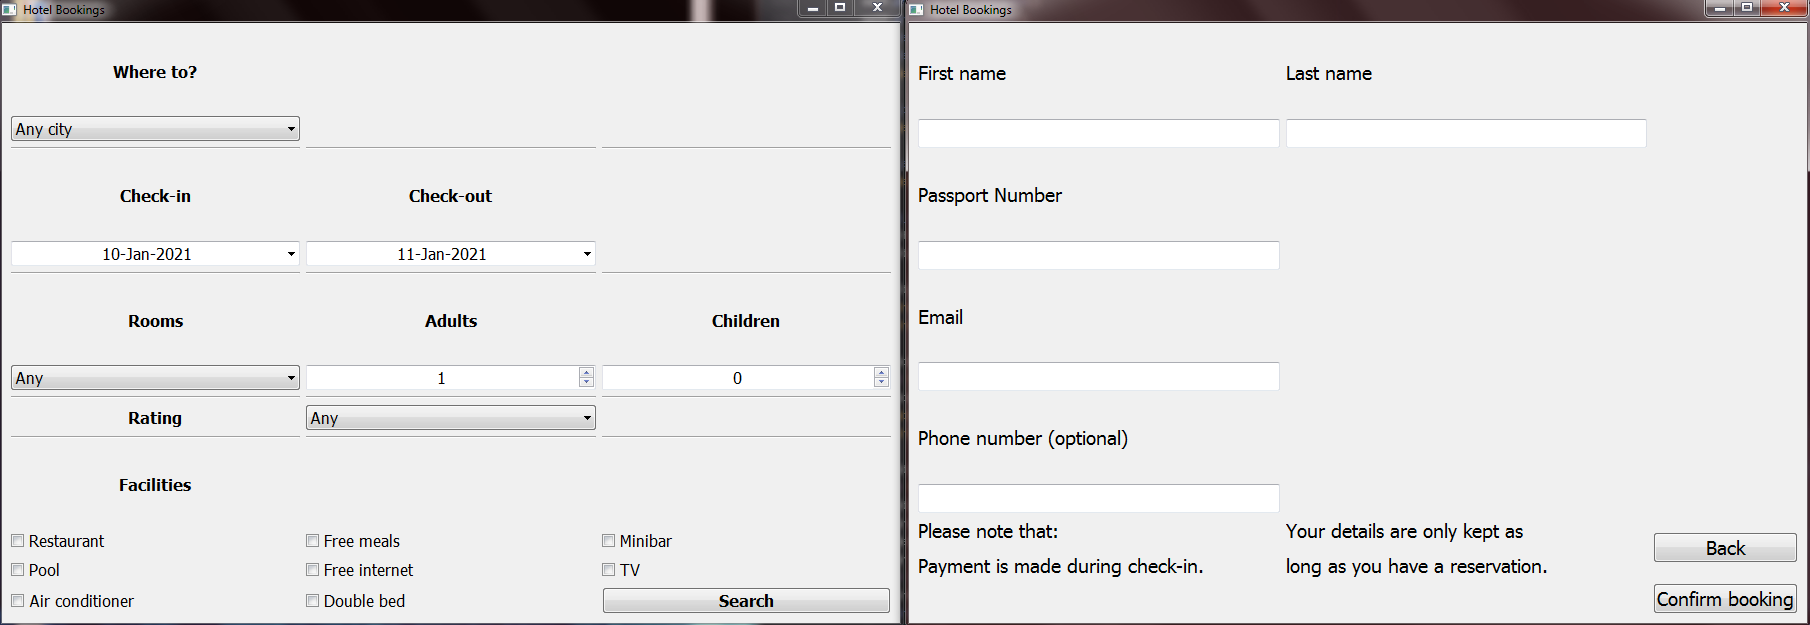
\includegraphics[width=\linewidth]{ClientInt.PNG}
	\caption{Interfață client.}\label{fig:fig2}
\end{figure}

\begin{figure}[!htb]
	\centering
	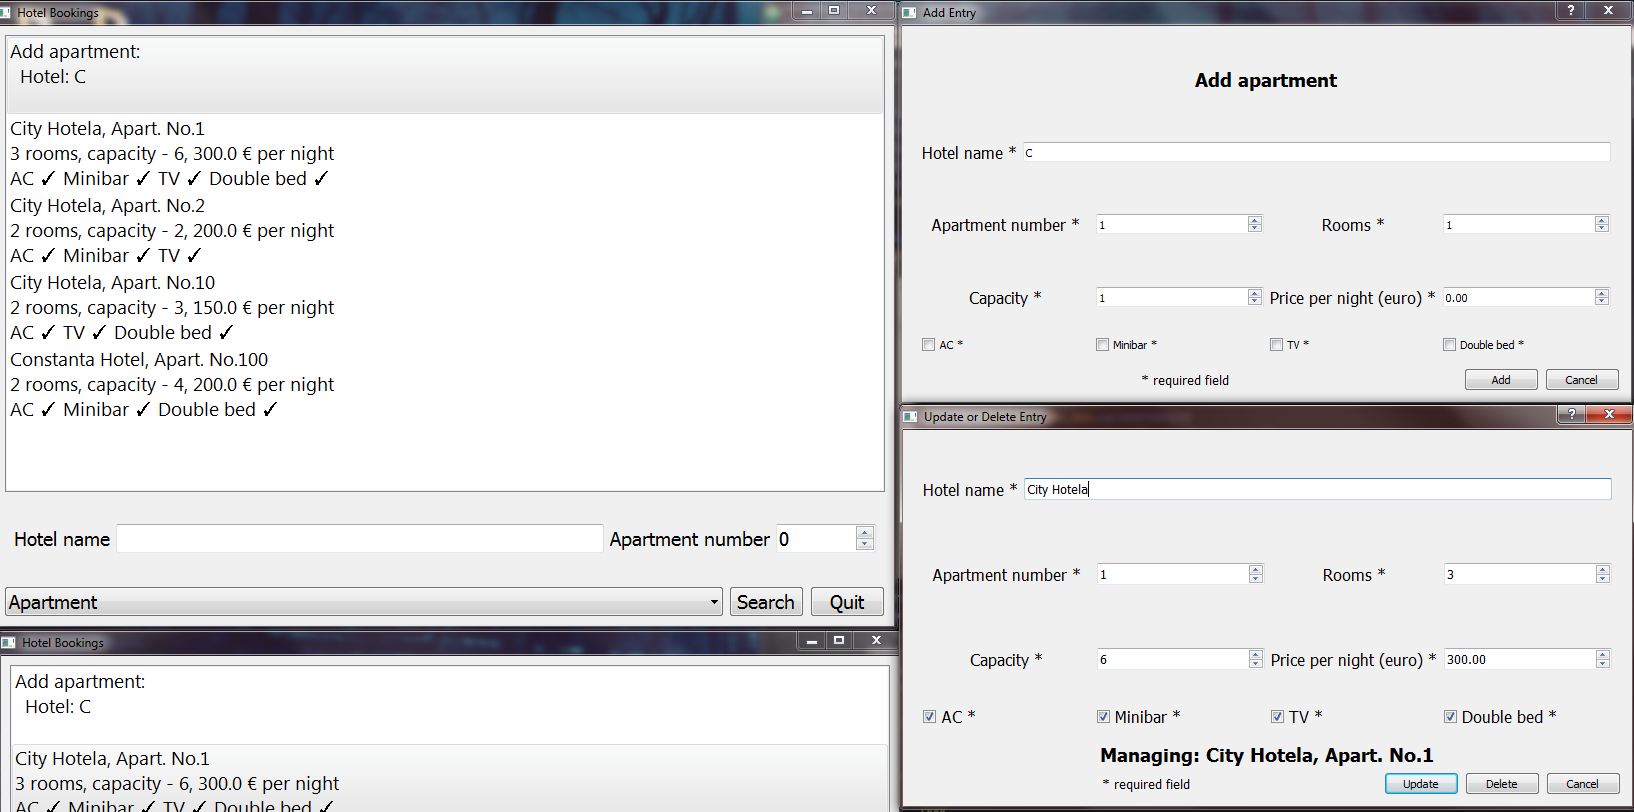
\includegraphics[width=\linewidth]{AdminInt.PNG}
	\caption{Interfață administrator.}\label{fig:fig3}
\end{figure}

\begin{figure}[!htb]
	\centering
	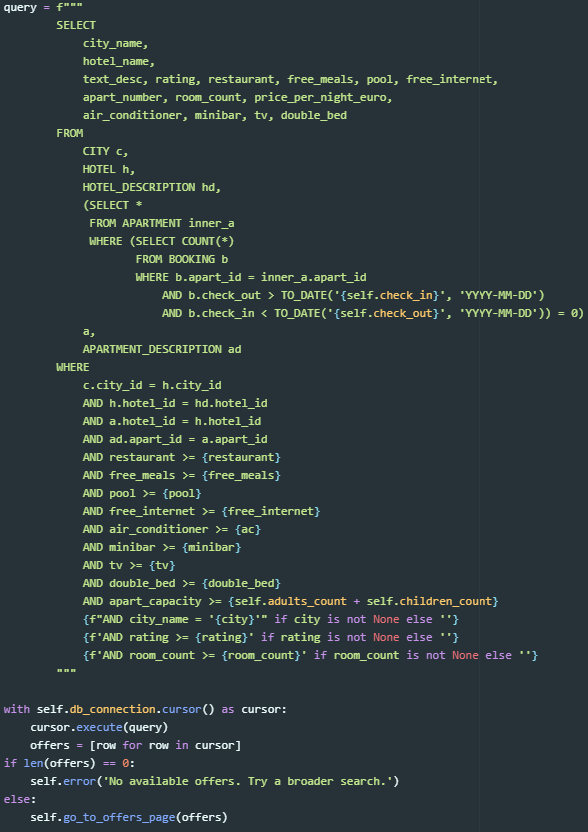
\includegraphics[width=\linewidth]{SearchEx.PNG}
	\caption{Exemplu interogare: căutare.}\label{fig:fig4}
\end{figure}

\end{document}